\section{Оборудование}
\begin{figure}[ht!]
    \center{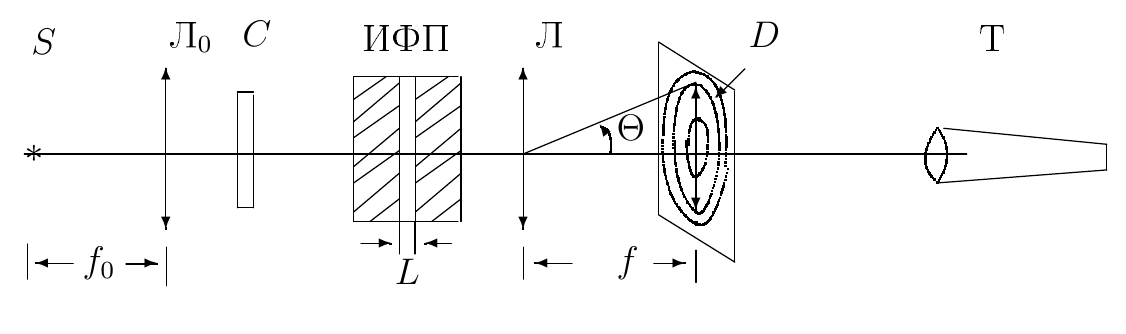
\includegraphics[width=0.8\linewidth]{../img/img1.png}}
\end{figure}

Схема экспериментальной установки представлена на рисунке. Свет от лампы S проходит через линзу $\text{Л}_{0}$ и светофильтр С и попадает на интерферометр Фабри-Перо. Линза $\text{Л}_{0}$ служит для формирования слегка расходящегося пучка лучей. Интерфереционные кольца наблюдаются в фокальной плоскости линзы Л. Картинка рассматривается через зрительную трубу Т, сфокусированную на эту плоскость. Диаметры колец измеряются с помощью микроскопа катетометра.
